%!TEX root = ../template.tex
%%%%%%%%%%%%%%%%%%%%%%%%%%%%%%%%%%%%%%%%%%%%%%%%%%%%%%%%%%%%%%%%%%%%
%% p_delta_scour_wall_validation.tex
%% Rigid-wall benchmark for P--Delta and scour implementation
%%%%%%%%%%%%%%%%%%%%%%%%%%%%%%%%%%%%%%%%%%%%%%%%%%%%%%%%%%%%%%%%%%%%

\section{Rigid-Wall Validation of the P--Delta and Scour Procedures}
\label{sec:wall-pdelta-scour-validation}

Before applying the scour procedure to a complete masonry arch bridge, a
controlled benchmark was developed to assess whether the numerical model
reproduces the expected overturning response of a wall--foundation system.
The benchmark has two complementary purposes. First, it verifies the
implementation of geometric nonlinearity in HiStrA by comparing a computed
rocking path with a closed-form rigid-body solution. Second, it verifies the
staged representation of scour, in which a prescribed part of the
soil--foundation interface is removed before an eccentric vertical load is
applied. The problem is deliberately simple enough to admit an analytical
solution, while retaining the contact discretisation, nonlinear solution
strategy and P--Delta implementation used in the bridge applications.

The validation follows the rationale adopted by Cusmano et al. \cite{Cusmano2023}, who
assessed the P--Delta formulation of the \gls{DMEM} against analytical
rigid-block solutions for rocking masonry walls. Their study demonstrated
that geometric nonlinearities are required to reproduce both the descending
branch and the displacement at which the stabilising contribution of gravity
vanishes. It also showed that a deformable interface generally predicts a
lower peak force than the ideal rigid-block solution, and that the numerical
response approaches the rigid limit as the interface stiffness and fibre
discretisation are increased. The present benchmark extends that validation
concept to a changing foundation-support geometry caused by scour.

\subsection{Benchmark geometry and discretisation}
\label{sec:wall-validation-geometry}

The model comprises a rectangular foundation and a centred masonry wall. The
foundation is $2.88$~m wide in the rocking direction, $1.398$~m long and
$0.758$~m deep. The wall is $2.88$~m wide, $0.44$~m thick and $1.495$~m high.
The eccentric vertical load acts at the negative edge of the wall,
$y_L=-1.44$~m, at an elevation of $H_2=2.253$~m above the foundation base.
The principal geometric and gravitational quantities are summarised in
\Cref{tab:wall-validation-components}.

\begin{figure}[htbp]
\centering
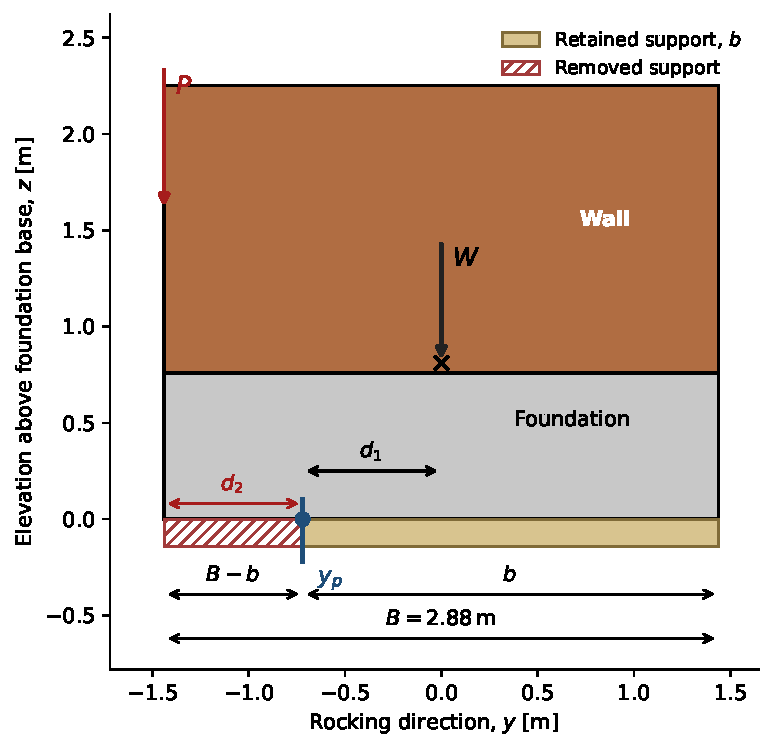
\includegraphics[width=0.82\linewidth]{./Figures/wall_pdelta_scour_geometry.pdf}
\caption{Rigid-wall benchmark in the rocking plane, showing the retained
support, removed contact, ideal pivot and moment arms. The illustrated
support ratio is representative; all six ratios are analysed.}
\label{fig:wall-validation-geometry}
\end{figure}

\begin{table}[htbp]
\centering
\caption{Geometry, weight and centroid of the rigid-wall benchmark.}
\label{tab:wall-validation-components}
\begin{tabular}{lcccc}
\hline
Component & Dimensions (m) & Volume (m$^3$) & Weight (kN) & $z_G$ above base (m)\\
\hline
Foundation & $1.398\times2.880\times0.758$ & 3.051890 & 68.362334 & 0.379000\\
Wall       & $0.440\times2.880\times1.495$ & 1.894464 & 42.435994 & 1.505500\\
\hline
Total/centroid & -- & 4.946354 & 110.798328 & 0.810452\\
\hline
\end{tabular}
\end{table}

The numerical model contains 336 spatial macro-elements and 2352 global
degrees of freedom. The base of the foundation is connected to restraints by
72 interface patches, arranged in six patches across the foundation length.
Each patch is discretised by a $9\times9$ grid of normal links. In the region
considered for scour, consecutive interface rows are 0.18~m wide; removal of
one to six rows therefore produces the six support ratios considered below.
This discretisation is important because the rigid solution assumes a pivot
exactly at the scour front, whereas the numerical contact reaction is
distributed over a finite set of compressive links.

The foundation contact is assigned a no-tension, compression-transmitting
material denoted as \emph{Soil}. In the final validation model, the
longitudinal and transverse elastic moduli are both set to
$10{,}000$~MPa. The tensile strength is reduced to a negligible value so that
uplift can occur, while the retained compressive links provide an
approximately rigid unilateral support. The \emph{Soil\_removed} material has
an elastic modulus of $0.005$~MPa and negligible tensile and compressive
strength. It consequently contributes no meaningful support after a scour
stage. The relevant properties are listed in
\Cref{tab:wall-validation-contact-materials}.

\begin{table}[htbp]
\centering
\caption{Interface properties used in the rigid-wall validation model.}
\label{tab:wall-validation-contact-materials}
\begin{tabular}{lcccc}
\hline
Material & $E_{\mathrm{hor}}$ (MPa) & $E_{\mathrm{ver}}$ (MPa)
& $f_{c,\mathrm{hor}}$ (MPa) & $f_{t,\mathrm{hor}}$ (MPa)\\
\hline
Soil & 10000 & 10000 & 0.03 & $10^{-8}$\\
Soil removed & 0.005 & 0.005 & $10^{-8}$ & $10^{-8}$\\
\hline
\end{tabular}
\end{table}

These values should not be interpreted as a site-specific geotechnical soil
model. They define a quasi-rigid unilateral contact used for verification of
the numerical formulation. This distinction is essential: the benchmark
tests whether HiStrA reproduces a prescribed rigid-body limit, whereas the
bridge application in \Cref{sec:dmem-scour-foundation} adopts a separate
soil--foundation calibration appropriate to that structural model.

\subsection{Analytical rocking solution}
\label{sec:wall-validation-analytical}

Let $B=2.88$~m be the total foundation width and $b$ the width that remains
supported after scour. The retained support ratio is

\begin{equation}
\rho_b=\frac{b}{B}.
\label{eq:wall-validation-support-ratio}
\end{equation}

Scour advances from the negative-$y$ edge, coincident with the vertical load
line. With the origin at the centre of the wall, the ideal pivot is located at

\begin{equation}
y_p=-\frac{B}{2}+(B-b)=B\left(\frac{1}{2}-\rho_b\right).
\label{eq:wall-validation-pivot}
\end{equation}

Since the weight centroid is at $y_G=0$, the lever arms of the self-weight and
live load in the undeformed configuration are, respectively,

\begin{equation}
d_1=y_G-y_p=B\left(\rho_b-\frac{1}{2}\right),
\qquad
d_2=y_p-y_L=B(1-\rho_b).
\label{eq:wall-validation-arms}
\end{equation}

Moment equilibrium about the pivot gives the rigid-body activation load

\begin{equation}
P_{\mathrm{cr}}=W\frac{d_1}{d_2}
=W\frac{\rho_b-0.5}{1-\rho_b},
\qquad \rho_b>0.5,
\label{eq:wall-validation-critical-load}
\end{equation}

where $W=110.798328$~kN is the combined weight of the wall and foundation.
Equation~\eqref{eq:wall-validation-critical-load} is an upper-bound reference
for the deformable numerical model because it assumes an immovable point
pivot and a perfectly rigid wall--foundation assembly.

After rocking begins, the vertical directions of $W$ and $P$ remain fixed in
the global reference system, while their moment arms change with the rotation
$\theta$. The corresponding equilibrium path is

\begin{equation}
P(\theta)=W\,
\frac{d_1\cos\theta-H_1\sin\theta}
{d_2\cos\theta+H_2\sin\theta},
\label{eq:wall-validation-rotation-path}
\end{equation}

where $H_1=0.810452$~m is the height of the combined weight centroid and
$H_2=2.253$~m is the elevation of the applied live load. The zero-load
configuration is reached when the weight resultant passes through the pivot,
giving

\begin{equation}
\theta_0=\tan^{-1}\left(\frac{d_1}{H_1}\right).
\label{eq:wall-validation-zero-rotation}
\end{equation}

For comparison with the numerical kinematics, the displacement of the loaded
point is measured relative to the translating pivot. If $d_{2,t}$ is the
horizontal distance between the pivot and the monitored point in the initial
configuration, its outward and downward displacements are

\begin{align}
u_y(\theta)&=H_2\sin\theta-d_{2,t}(1-\cos\theta),
\label{eq:wall-validation-horizontal-displacement}\\
u_z(\theta)&=d_{2,t}\sin\theta+H_2(1-\cos\theta).
\label{eq:wall-validation-vertical-displacement}
\end{align}

The scenario-specific analytical quantities are reported in
\Cref{tab:wall-validation-scenarios}. The large value of
$P_{\mathrm{cr}}$ for $\rho_b=0.9375$ results from the very short live-load
arm, $d_2=0.18$~m. Consequently, this scenario is especially sensitive to any
finite width or translation of the numerical contact resultant.

\begin{table}[htbp]
\centering
\caption{Analytical quantities for the six foundation-support scenarios.}
\label{tab:wall-validation-scenarios}
\begin{tabular}{ccccccc}
\hline
Rows removed & $b/B$ & $y_p$ (m) & $d_1$ (m) & $d_2$ (m)
& $P_{\mathrm{cr}}$ (kN) & $\theta_0$ ($^\circ$)\\
\hline
1 & 0.9375 & -1.260 & 1.260 & 0.180 & 775.588 & 57.250\\
2 & 0.8750 & -1.080 & 1.080 & 0.360 & 332.395 & 53.115\\
3 & 0.8125 & -0.900 & 0.900 & 0.540 & 184.664 & 47.997\\
4 & 0.7500 & -0.720 & 0.720 & 0.720 & 110.798 & 41.618\\
5 & 0.6875 & -0.540 & 0.540 & 0.900 &  66.479 & 33.675\\
6 & 0.6250 & -0.360 & 0.360 & 1.080 &  36.933 & 23.951\\
\hline
\end{tabular}
\end{table}

\subsection{P--Delta implementation in HiStrA}
\label{sec:wall-validation-pdelta-implementation}

The complete \gls{DMEM} formulation is presented elsewhere in this thesis and
is not repeated here. Only the treatment of P--Delta effects used in the
benchmark is summarised. HiStrA follows the computationally efficient
formulation proposed by Cusmano et al. \cite{Cusmano2023}: equilibrium is expressed with
respect to the undeformed model topology, and geometric effects are introduced
through an additional load vector rather than through the assembly of a
geometric stiffness matrix.

For a force distribution $\mathbf{f}$ acting on a macro-element, the
second-order moment is obtained from the displacement of its application
point relative to the macro-element centroid $G$,

\begin{equation}
\mathbf{M}_{P\Delta}^{(f)}=
\int_A\left[\mathbf{u}(\mathbf{x})-\mathbf{u}_G\right]
\times\mathbf{f}(\mathbf{x})\,\mathrm{d}A.
\label{eq:wall-validation-pdelta-external}
\end{equation}

The same operation is applied to the resultants $\mathbf{P}_j$ transmitted by
the interfaces,

\begin{equation}
\mathbf{M}_{P\Delta}^{(i)}=
\sum_j\left[\mathbf{u}(\mathbf{x}_j)-\mathbf{u}_G\right]
\times\mathbf{P}_j.
\label{eq:wall-validation-pdelta-interface}
\end{equation}

In the HiStrA implementation, the relative displacement is evaluated from the
current macro-element rotation $\boldsymbol{\phi}_G$ and the initial lever
vector $\mathbf{r}$, such that
$\Delta\mathbf{u}\simeq\boldsymbol{\phi}_G\times\mathbf{r}$. Contributions
from the applied line loads and from the resultants of the perimeter
interfaces are summed. The resulting moment is assembled into the rotational
degrees of freedom through

\begin{equation}
\mathbf{P}_{q,e}=
\begin{bmatrix}
0&0&0&M_{P\Delta,x}&M_{P\Delta,y}&M_{P\Delta,z}&0
\end{bmatrix}^{\mathsf{T}}.
\label{eq:wall-validation-pdelta-vector}
\end{equation}

The nonlinear residual therefore includes the conventional external load,
the second-order vector and the internal resisting force,

\begin{equation}
\mathbf{r}=\mathbf{f}_{\mathrm{ext}}+\mathbf{P}_q-
\mathbf{f}_{\mathrm{int}}.
\label{eq:wall-validation-residual}
\end{equation}

The live-load analysis uses the HiStrA option \texttt{EachStep}; hence the
P--Delta vector is recalculated at the beginning of every arc-length step from
the current committed configuration and interface resultants. HiStrA also
provides an \texttt{EachIteration} option, but it is not required for the
present benchmark. The adopted procedure retains the principal advantage
identified by Cusmano et al. \cite{Cusmano2023}: large-displacement rocking effects are
introduced with a small computational overhead and without reformulating the
macro-element tangent stiffness.

\subsection{Staged numerical procedure}
\label{sec:wall-validation-procedure}

Each scenario is analysed through the following sequence:

\begin{enumerate}
    \item all foundation-restraint interfaces are assigned the \emph{Soil}
    material and the self-weight is applied in the five-step \texttt{Vert}
    analysis;
    \item between one and six interface rows are changed to
    \emph{Soil\_removed}, and a five-step zero-load \texttt{scour\_1}
    analysis establishes equilibrium under the modified support condition;
    \item the eccentric vertical line load is applied in
    \texttt{LiveLoad\_1}. The physical live load is obtained from the load
    multiplier $\lambda$ as $P=0.44\lambda$~kN;
    \item the peak and descending branches are followed using arc-length
    control, with P--Delta effects updated at every committed step.
\end{enumerate}

The ascending path is controlled through the projected displacement of the
loaded point, using a maximum predictor increment of 25~kN and a control
radius of 0.05~cm around the peak. After a confirmed load reduction of
0.25~kN, the continuation coordinate is changed to the outward displacement
of the loaded point relative to the moving scour-front pivot. This avoids
using the vertical displacement as the sole post-peak coordinate, which is
ill-conditioned when the monitored point lies close to the pivot. The
remaining theoretical outward displacement is initially divided into 100
increments. If a trial diverges, its complete state is restored and the
arc-length radius is reduced by a factor of two, down to 0.05~cm. A maximum of
six cutbacks is permitted.

All three stages use the \texttt{ForceMoment} convergence criterion with a
tolerance of $10^{-4}$. In addition, every candidate step is subjected to an
independent global-equilibrium audit before commitment. The maximum permitted
global force imbalance is the greater of 0.05~kN and $10^{-5}$ of the current
force scale. A failed trial is never retained as structural response data.
This safeguard is particularly important in the post-peak range, where an
energy- or work-based scalar criterion may become small even when the system
is not adequately equilibrated.

\subsection{Peak-load comparison}
\label{sec:wall-validation-results}

The analytical and numerical peak loads are compared in
\Cref{tab:wall-validation-results}. Every numerical maximum is internal to
the computed path and is followed by at least one lower-load equilibrium
state. The peak is therefore not a truncation bound. HiStrA underestimates the
rigid-body prediction by 2.85--7.78\%, with a mean absolute percentage error
of 4.09\%. Across the full range of capacities, the coefficient of
determination between the analytical and numerical peaks is
$R^2=0.990$.

\begin{table}[htbp]
\centering
\caption{Rigid-body and HiStrA peak loads for the six support ratios.}
\label{tab:wall-validation-results}
\begin{tabular}{cccccc}
\hline
$b/B$ & $P_{\mathrm{cr,theory}}$ (kN) & $P_{\mathrm{cr,HiStrA}}$ (kN)
& Error (\%) & Committed steps & Zero load reached\\
\hline
0.9375 & 775.588 & 715.283 & -7.78 &  58 & No\\
0.8750 & 332.395 & 318.968 & -4.04 &  56 & No\\
0.8125 & 184.664 & 178.884 & -3.13 &  70 & No\\
0.7500 & 110.798 & 107.644 & -2.85 & 104 & Yes\\
0.6875 &  66.479 &  64.488 & -3.00 & 136 & No\\
0.6250 &  36.933 &  35.540 & -3.77 & 135 & Yes\\
\hline
\end{tabular}
\end{table}

\begin{figure}[htbp]
\centering
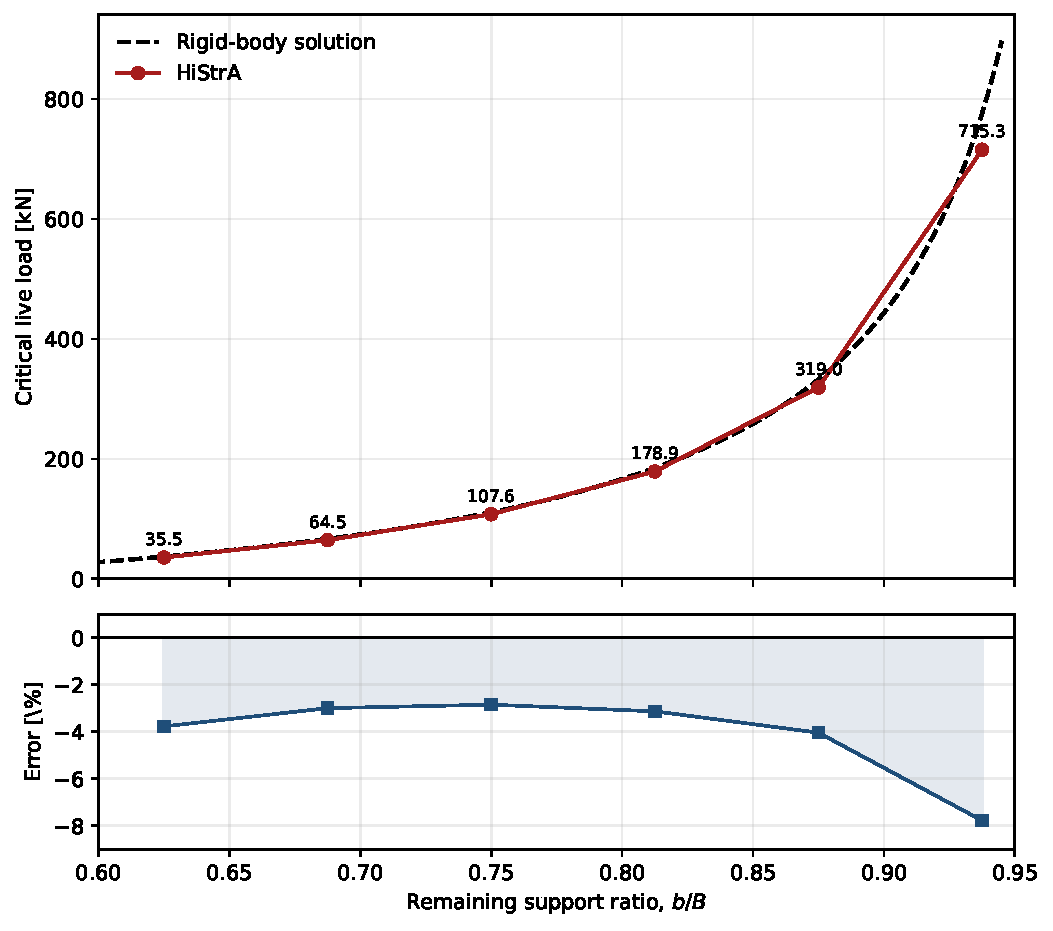
\includegraphics[width=0.78\linewidth]{./Figures/wall_pdelta_scour_capacity.pdf}
\caption{Comparison between the rigid-body critical load and the HiStrA peak
load for the six retained-support ratios. The lower panel shows the relative
error with respect to the analytical solution.}
\label{fig:wall-validation-capacity}
\end{figure}

The agreement confirms that the staged removal of the contact rows produces
the intended variation of the pivot position and of the stabilising and
overturning moment arms. It also confirms the expected nonlinear trend: the
capacity decreases rapidly as the scour front approaches the weight
resultant. The small systematic underestimation is mechanically consistent
with the findings of Cusmano et al. \cite{Cusmano2023}. The rigid-body solution concentrates
the reaction at a geometric point on an undeformable base. Conversely,
the HiStrA contact has finite stiffness and its compressive resultant acts
over a finite group of links inside the remaining support. The foundation and
wall also retain finite deformability.

The largest discrepancy occurs for $b/B=0.9375$. In that case, $d_2$ is only
0.18~m, so a small inward displacement of the effective contact resultant
causes a comparatively large change in the moment ratio $d_1/d_2$. This
explains why the error increases even though the absolute support
discretisation is unchanged. Increasing the longitudinal and transverse
moduli of the retained contact improved the agreement substantially, as
expected from the stiffness study reported by Cusmano et al. \cite{Cusmano2023}. The final
values of $10{,}000$~MPa should therefore be understood as a quasi-rigid
benchmark calibration rather than as an independently measured soil modulus.

\subsection{Post-peak response and validation limits}
\label{sec:wall-validation-postpeak}

All six analyses develop a descending branch after the maximum load. This is
the principal qualitative signature of the P--Delta formulation: as rocking
increases, the horizontal lever arm of the stabilising weight progressively
decreases, and the load required to maintain equilibrium tends towards zero.
The numerical tilt--load curves follow the analytical softening trend, while
the comparison of horizontal and vertical displacements shows the influence
of contact compliance, pivot translation and macro-element deformation that
is absent from the rigid-body model.

\begin{figure}[htbp]
\centering
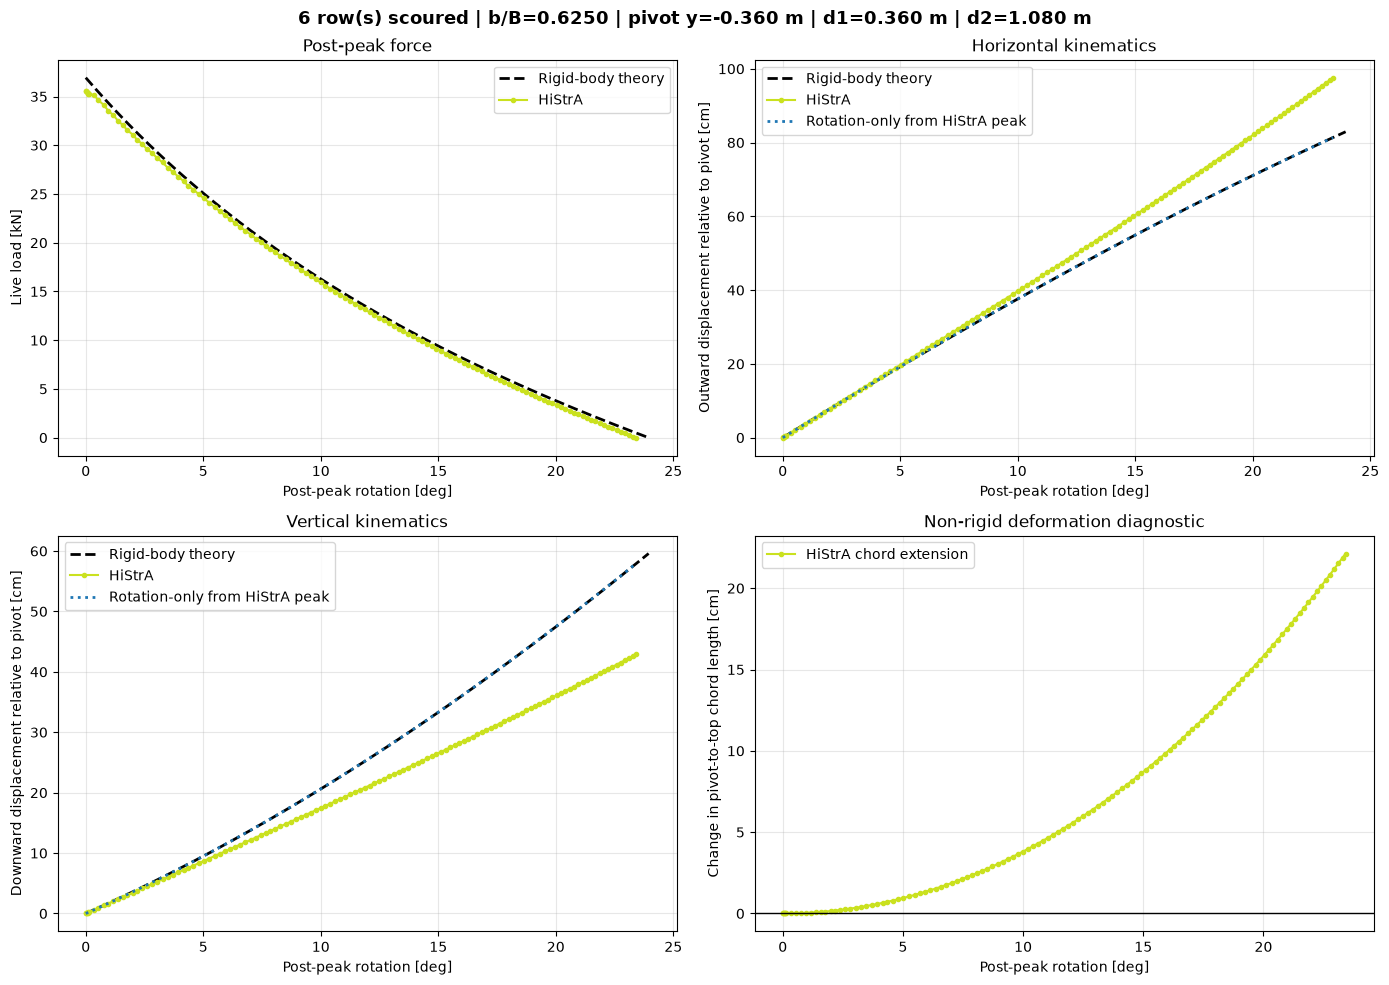
\includegraphics[width=0.98\linewidth]{./Figures/wall_pdelta_scour_postpeak_0625.png}
\caption{Post-peak response for $b/B=0.6250$. Displacements are measured at
the loaded point relative to the moving scour-front pivot. The
rotation-only curves apply rigid kinematics to the HiStrA configuration at
peak load, whereas the solid numerical curves include the deformation of the
wall--foundation assembly.}
\label{fig:wall-validation-postpeak-0625}
\end{figure}

The complete $b/B=0.6250$ response in
\Cref{fig:wall-validation-postpeak-0625} illustrates both the capability and
the limits of the comparison. The live-load--rotation curve remains close to
the analytical solution until the load returns to zero, supporting the
P--Delta equilibrium formulation. The rotation-only displacement curves also
closely reproduce the analytical kinematic transformation. The actual HiStrA
response, however, develops greater outward displacement and smaller downward
displacement. The simultaneous increase of the pivot-to-top chord length
shows that the numerical assembly is not behaving as a perfectly rigid block
at large rotation. The displacement discrepancy is therefore associated with
contact translation and structural deformation, rather than with the
trigonometric rigid-body transformation itself.

Zero live load is reached explicitly for $b/B=0.7500$ and $0.6250$. For the
other four cases, a valid descending sequence is obtained, but the nonlinear
continuation terminates before the theoretical zero-load configuration. The
termination follows repeated failures of reduced-radius trials; those trial
states are rolled back and are not included in
\Cref{tab:wall-validation-results}. Accordingly, the present study provides
stronger validation of the scour-dependent peak capacity than of the complete
ultimate-displacement path.

This limitation is most pronounced when the retained contact reduces to a
small rocking and sliding region. In that range, the tangent system approaches
a mechanism and a single scalar displacement coordinate may not uniquely
control all foundation translations and rotations. Increasing the maximum
displacement or accepting a weak work criterion would allow non-equilibrated
states to enter the response and is therefore not an acceptable remedy.
Continuation to the analytical zero-load point would require either a more
general multiparameter path-following procedure or an additional kinematic
restraint at the pivot. The latter would alter the physical model and was not
introduced in this validation.

\subsection{Validation outcome}
\label{sec:wall-validation-conclusions}

The benchmark supports the following conclusions:

\begin{enumerate}
    \item the staged replacement of \emph{Soil} by
    \emph{Soil\_removed} correctly moves the active support boundary in
    0.18~m increments;
    \item the numerical peak capacities reproduce the analytical dependence
    on $b/B$ with a mean absolute percentage error of approximately 4.1\%;
    \item the remaining difference from the analytical limit is consistent
    with finite contact stiffness, finite fibre spacing and deformation of
    the wall--foundation assembly;
    \item the stepwise P--Delta load-vector update reproduces the expected
    descending rocking response without assembling a geometric stiffness
    matrix, consistently with the formulation validated by
    Cusmano et al. \cite{Cusmano2023};
    \item the independent equilibrium audit and failed-step rollback are
    necessary for a physically admissible interpretation of the post-peak
    response; and
    \item peak-load agreement is demonstrated for all six scour scenarios,
    whereas complete zero-load displacement validation is presently limited
    to two scenarios.
\end{enumerate}

The wall benchmark therefore provides a transparent intermediate validation
between the analytical rigid-body problem and the complete bridge models. It
demonstrates that the numerical procedure captures the coupled effects of
support loss, unilateral contact and geometric nonlinearity, while also
identifying the range in which the ideal rigid-pivot assumption ceases to be
representative of the deformable numerical model.
